\begin{figure}
      \begin{subfigure}{1.0\textwidth}
  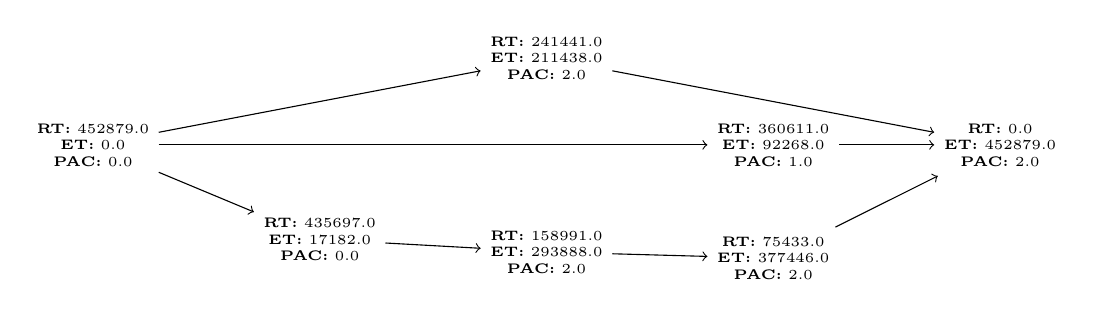
\begin{tikzpicture}
      \draw[align=center,font=\tiny]
        (-12.24, 1.98) node (0){\textbf{RT:} 452879.0\\\textbf{ET:} 0.0\\\textbf{PAC:} 0.0}
        (-9.36, 0.78) node (1){\textbf{RT:} 435697.0\\\textbf{ET:} 17182.0\\\textbf{PAC:} 0.0}
        (-3.6, 1.98) node (2){\textbf{RT:} 360611.0\\\textbf{ET:} 92268.0\\\textbf{PAC:} 1.0}
        (-6.48, 3.08) node (3){\textbf{RT:} 241441.0\\\textbf{ET:} 211438.0\\\textbf{PAC:} 2.0}
        (-6.48, 0.62) node (4){\textbf{RT:} 158991.0\\\textbf{ET:} 293888.0\\\textbf{PAC:} 2.0}
        (-3.6, 0.54) node (5){\textbf{RT:} 75433.0\\\textbf{ET:} 377446.0\\\textbf{PAC:} 2.0}
        (-0.72, 1.98) node (6){\textbf{RT:} 0.0\\\textbf{ET:} 452879.0\\\textbf{PAC:} 2.0};
      \begin{scope}[->]
        \draw (0) to (1);
        \draw (0) to (2);
        \draw (0) to (3);
        \draw (1) to (4);
        \draw (2) to (6);
        \draw (3) to (6);
        \draw (4) to (5);
        \draw (5) to (6);
      \end{scope}
    \end{tikzpicture}

  \end{subfigure}
  \begin{subfigure}{1.0\textwidth}
  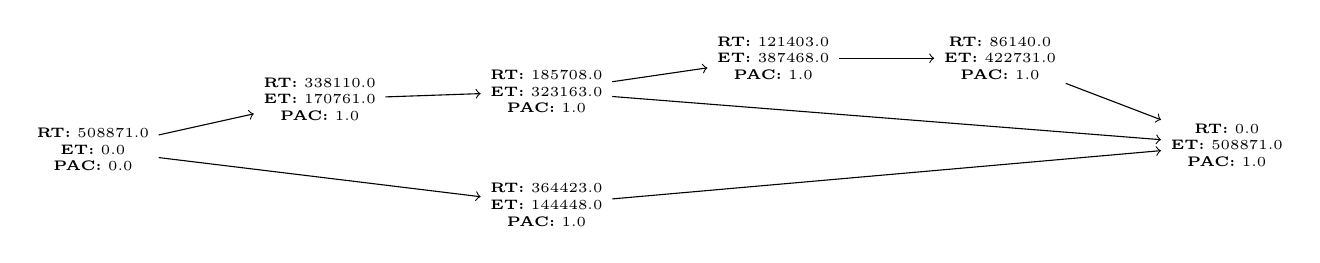
\begin{tikzpicture}
      \draw[align=center,font=\tiny]
        (-15.12, 1.24) node (7){\textbf{RT:} 508871.0\\\textbf{ET:} 0.0\\\textbf{PAC:} 0.0}
        (-9.36, 0.54) node (8){\textbf{RT:} 364423.0\\\textbf{ET:} 144448.0\\\textbf{PAC:} 1.0}
        (-12.24, 1.88) node (9){\textbf{RT:} 338110.0\\\textbf{ET:} 170761.0\\\textbf{PAC:} 1.0}
        (-9.36, 1.98) node (10){\textbf{RT:} 185708.0\\\textbf{ET:} 323163.0\\\textbf{PAC:} 1.0}
        (-6.48, 2.4) node (11){\textbf{RT:} 121403.0\\\textbf{ET:} 387468.0\\\textbf{PAC:} 1.0}
        (-3.6, 2.4) node (12){\textbf{RT:} 86140.0\\\textbf{ET:} 422731.0\\\textbf{PAC:} 1.0}
        (-0.72, 1.3) node (13){\textbf{RT:} 0.0\\\textbf{ET:} 508871.0\\\textbf{PAC:} 1.0};
      \begin{scope}[->]
        \draw (7) to (8);
        \draw (7) to (9);
        \draw (8) to (13);
        \draw (9) to (10);
        \draw (10) to (11);
        \draw (10) to (13);
        \draw (11) to (12);
        \draw (12) to (13);
      \end{scope}
    \end{tikzpicture}

  \end{subfigure}
    
  \caption{Feature graphs}
    \label{fig:feature-graphs}
\end{figure}
